\chapter[第三章]{} % (fold)
\label{cha:chapter3}

\section{问题 \\ 列主元 Gauss 消去}

对于某电路的分析,归结于求解线性方程组 $RI = V$,其中

$$
R = 
\begin{bmatrix}
31 & -13 & 0 & 0 & 0 & -10 & 0 & 0 & 0 \\
-13 & 35 & -9 & 0 & -11 & 0 & 0 & 0 & 0 \\
0 & -9 & 31 & -10 & 0 & 0 & 0 & 0 & 0 \\
0 & 0 & -10 & 79 & -30 & 0 & 0 & 0 & -9 \\
0 & 0 & 0 & -30 & 57 & -7 & 0 & -5 & 0 \\
0 & 0 & 0 & 0 & -7 & 47 & -30 & 0 & 0 \\
0 & 0 & 0 & 0 & 0 & -30 & 41 & 0 & 0 \\
0 & 0 & 0 & 0 & -5 & 0 & 0 & 27 & -2 \\
0 & 0 & 0 & -9 & 0 & 0 & 0 & -2 & 29
\end{bmatrix}
$$

$$
V^T = (-15, 27, -23, 0, -20, 12, -7, 7, 10)^T
$$

\begin{enumerate}
    \item 编制解 n 阶线性方程组 $Ax = b$ 的列主元 Gauss 消去的通用程序;

    \item 用所编程序解线性方程组 $RI = V$,并打印出解向量,保留5位有效数字;

    \item 本题编程之中,你提高了哪些能力?

\end{enumerate}

\section{分析}

列主元 Gauss 消去的算法流程图如图 \ref{fig:GaussFlow} 所示。

  \begin{figure}[ht]
  \centering
    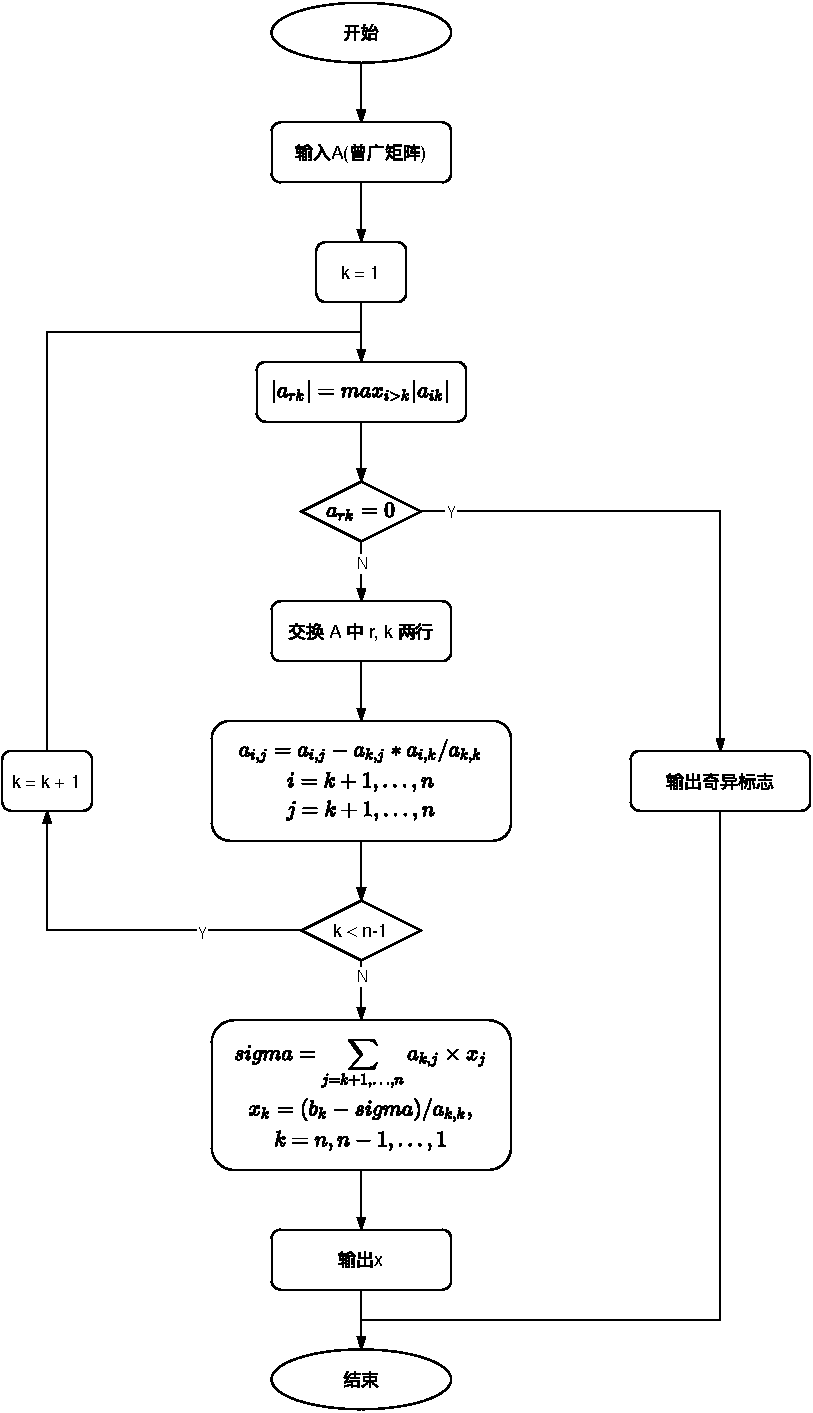
\includegraphics[width=0.7\textwidth]{GaussFlow}
    \caption{列主元 Gauss 消去算法流程}
    \label{fig:GaussFlow}
  \end{figure}

\section{程序}

\begin{lstlisting}[style = python]
import sys
import numpy as np

A = [[31, -13, 0, 0, 0, -10, 0, 0, 0],
    [-13, 35, -9, 0, -11, 0, 0, 0, 0],
    [0, -9, 31, -10, 0, 0, 0, 0, 0],
    [0, 0, -10, 79, -30, 0, 0, 0, -9],
    [0, 0, 0, -30, 57, -7, 0, -5, 0],
    [0, 0, 0, 0, -7, 47, -30, 0, 0],
    [0, 0, 0, 0, 0, -30, 41, 0, 0],
    [0, 0, 0, 0, -5, 0, 0, 27, -2],
    [0, 0, 0, -9, 0, 0, 0, -2, 29]]

b = [-15, 27, -23, 0, -20, 12, -7, 7, 10]

def find_shape(A, b):
    """
    获取 n
    """

    # n行 m列
    n1, m1 = A.shape
    n2, = b.shape

    # print(n1, m1)
    # print(n2)

    # 判断矩阵形状
    if n1 != m1 or n1 != n2:
        print('Error martix shape!')
        sys.exit()
    else:
        N = n1

    return N
    

def MGauss(A, b):
    """
    列主元 Gauss 消去 消元
    """

    # 判断矩阵形状
    N = find_shape(A, b)

    # 列主元高斯消元
    for k in range(0, N):
        p = k
        maxabs = abs(A[k, k])
        # 找列最大值
        for i in range(k+1, N):
            if abs(A[i, k]) > maxabs:
                p = i
                maxabs = abs(A[i, k])
        print('maxabs', maxabs)
        # 最大值为 0
        if maxabs == 0:
            print('Singular')
            sys.exit()
        # 最大值不在对角线, 则交换两行
        if p != k:
            A[[p,k],:] = A[[k,p],:]
            b[[p,k]] = b[[k,p]]
        print('exchange r{0} and r{1}:\r\n'.format(k, p), A)
        # 消元,将对角线以下变为 0
        for i in range(k+1, N):
            m_ik = A[i, k] / A[k, k]
            for j in range(0, N):
                A[i, j] -= A[k, j] * m_ik
            b[i] -= b[k] * m_ik
        print('After Elimination:\r\n', np.concatenate((A,np.asarray([b]).T), axis = 1))
        
    if A[N-1, N-1] == 0:
        print('Singular')
        sys.exit()
    
    return A, b
        
def bring_back(A, b):
    """
    列主元 Gauss 消去 回带
    """
    
    # 判断矩阵形状
    N = find_shape(A, b)

    # 回带
    X = np.zeros(N)
    X[N-1] = b[N-1] / A[N-1, N-1]
    for i in range(0, N-1):
        k = N-2-i
        sigma = sum(A[k, j]*X[j] for j in range(k+1, N))
        # print('k:{0}, sigma:{1}'.format(k, sigma))
        X[k] = (b[k] - sigma) / A[k, k]

    return X
        
def main():
    """
    main
    """

    A_np = np.asarray(A, dtype = float)
    b_np = np.asarray(b, dtype = float)

    # b_np = b_np.T

    print('A:\r\n', A_np)
    print('b:\r\n', b_np)

    A_G, b_G = MGauss(A_np, b_np)
    x_G = bring_back(A_G, b_G)

    print('A_G:b_G\r\n', np.concatenate((A_G,np.asarray([b_G]).T), axis = 1))
    print('x_G', x_G)


if __name__ == "__main__":
    main()
\end{lstlisting}

\section{算例}

$$
A = 
\begin{bmatrix}
31 & -13 & 0 & 0 & 0 & -10 & 0 & 0 & 0 \\
-13 & 35 & -9 & 0 & -11 & 0 & 0 & 0 & 0 \\
0 & -9 & 31 & -10 & 0 & 0 & 0 & 0 & 0 \\
0 & 0 & -10 & 79 & -30 & 0 & 0 & 0 & -9 \\
0 & 0 & 0 & -30 & 57 & -7 & 0 & -5 & 0 \\
0 & 0 & 0 & 0 & -7 & 47 & -30 & 0 & 0 \\
0 & 0 & 0 & 0 & 0 & -30 & 41 & 0 & 0 \\
0 & 0 & 0 & 0 & -5 & 0 & 0 & 27 & -2 \\
0 & 0 & 0 & -9 & 0 & 0 & 0 & -2 & 29
\end{bmatrix}
$$

$$
b^T = (-15, 27, -23, 0, -20, 12, -7, 7, 10)^T
$$

运算结果:

\begin{lstlisting}[style = python]
x_G [-0.28923382  0.34543572 -0.71281173 -0.22060851 -0.43040043  0.15430874 -0.05782287  0.20105389  0.29022866]
\end{lstlisting}

使用 MATLAB 自带的求解线性方程组的方法求解,验证编写算法的正确性:

\begin{lstlisting}[style = null]
>> A \ b'

ans =

   -0.2892
    0.3454
   -0.7128
   -0.2206
   -0.4304
    0.1543
   -0.0578
    0.2011
    0.2902
\end{lstlisting}

可以看到结果是一致的。

\section{结论}

\begin{enumerate}
    \item 列主元 Gauss 消去法避免了小数作除数,因此一般能保证舍入误差不增大,这个方法基本上是稳定的;

    \item MATLAB 中可用 \lstinline[style = null]| A \ b | 求线性方程组解。
\end{enumerate}

% chapter chapter1 (end)